\documentclass[12pt]{article}

% Language setting
\usepackage[english]{babel} 

% Set page size and margins
\usepackage[a4paper,top=3cm,bottom=3cm,left=2.5cm,right=2.5cm,marginparwidth=1.75cm]{geometry}

% Other useful packages
\usepackage{amsmath}
\usepackage{graphicx}
\usepackage[colorlinks=true, allcolors=blue]{hyperref}
\usepackage{listings}
\usepackage{xcolor}
\usepackage{enumitem}
\usepackage{verbatim}
\usepackage{tikz}
\usetikzlibrary{shapes,arrows,positioning}

% Code style settings
\lstset{
    language=Verilog,
    basicstyle=\ttfamily\small,
    keywordstyle=\color{blue}\bfseries,
    commentstyle=\color{green!60!black},
    stringstyle=\color{red},
    numbers=left,
    numberstyle=\tiny\color{gray},
    stepnumber=1,
    numbersep=5pt,
    backgroundcolor=\color{gray!10},
    frame=single,
    breaklines=true,
    breakatwhitespace=true,
    tabsize=2,
    showspaces=false,
    showstringspaces=false
}






\title{Team06 Lab3 Report}
\author{B12901193, B12901166, B12901030 Yu-Siang Huang}

\begin{document}
\maketitle

\begin{abstract}
This project implements a digital audio recording and playback system on FPGA (DE2-115 board) using WM8731 codec and I2S protocol. Audio data is stored in SRAM (1M × 16-bit, ~30 seconds at 32 kHz).

The system features variable-speed playback (1/8x to 8x) with constant and linear interpolation methods, and includes a robot voice effect using envelope following and Hadamard transform. A finite state machine manages system operation across seven states: idle, initialization, recording, playback, and their pause states.

The design utilizes multiple clock domains (12 MHz system, 100 kHz I2C, I2S bit clock) with proper synchronization. Experimental results demonstrate successful real-time audio processing with user-controllable speed and effects.

\textbf{Keywords:} FPGA, Digital Audio Processing, I2S Protocol, Variable Speed Playback
\end{abstract}

\section{File Structure}
\begin{verbatim}
team06_lab3/
|-- team06_lab3_report.pdf                    
|-- DE2_115.qsf                    # Quartus project settings file
|-- src/                           # Source code directory
|   |-- Top.sv                     # Top-level module (main state machine)
|   |-- I2cInitializer.sv          # I2C initialization for WM8731
|   |-- AudRecorder.sv             # I2S receiver (ADC input)
|   |-- AudDSP.sv                  # Digital signal processing module
|   |-- AudPlayer.sv               # I2S transmitter (DAC output)
|   |-- LCD.sv                     # LCD display controller
|   |-- Clean_sram.sv              # SRAM clearing module
|   |
|   |-- DE2_115/                   # Hardware interface layer
|
|-- qsys/                          # Qsys-generated files
\end{verbatim}



\section{System Architecture}

This is a digital audio recording and playback system implemented in the FPGA (DE2-115 development board). The system uses WM8731 audio codec for analog-to-digital conversion and SRAM as the audio data buffer. The system supports recording, playback, variable speed playback (fast/slow), and various audio effects processing.

\subsection{System Architecture Hierarchy}

\begin{verbatim}
+-------------------------------------------------------------+
|                      DE2_115.sv                             |
|            (Hardware Interface Layer / Top Module)          |
|  - Button inputs (KEY[3:0])                                 |
|  - Switch inputs (SW[17:0])                                 |
|  - LED outputs                                              |
|  - LCD outputs                                              |
|  - SRAM interface                                           |
|  - I2C interface (WM8731)                                   |
|  - I2S audio interface                                      |
|  - PLL clock generator (12MHz, 100kHz)                      |
+----------------------+--------------------------------------+
                       |
                       v
+-------------------------------------------------------------+
|                      Top.sv                                 |
|              (System Control Layer / State Machine)         |
|  - Main state machine (IDLE, I2C, RECD, RECD_PAUSE,         |
|    PLAY, PLAY_PAUSE)                                        |
|  - System initialization flow control                       |
|  - Record/Play mode switching                               |
|  - SRAM multiplexer control                                 |
+-----+-----------+-----------+-----------+-----------+-------+
      |           |           |           |           |
      v           v           v           v           v
+----------+ +----------+ +----------+ +----------+ +---------+
|  I2C     | | AudRec-  | |  AudDSP  | | AudPlayer| |   LCD   |
| Initial- | | order    | |          | |          | |         |
| izer     | |          | |          | |          | |         |
+----------+ +----------+ +----------+ +----------+ +---------+
      |           |           |           |           |
      v           v           v           v           v
+----------+ +----------+ +----------+ +----------+ +---------+
|  WM8731  | |   SRAM   | |   SRAM   | |  WM8731  | |   LCD   |
|  Codec   | |  (Write) | |  (Read)  | |   DAC    | | Display |
+----------+ +----------+ +----------+ +----------+ +---------+
\end{verbatim}

\subsection{Module Descriptions}

\subsubsection{DE2\_115.sv (Hardware Interface Layer)}

\paragraph{Function:} Connects FPGA with DE2-115 development board hardware resources

\noindent
\paragraph{Main Responsibilities:}
\begin{itemize}
    \item Button debouncing (\texttt{Debounce})
    \item PLL clock generation (\texttt{Altpll, generated from Qsys})
    \begin{itemize}
        \item \texttt{CLK\_12M}: 12 MHz (WM8731 master clock)
        \item \texttt{CLK\_100K}: 100 kHz (I2C clock)
    \end{itemize}
    \item Hardware signal routing to \texttt{Top.sv}
\end{itemize}

\noindent
\textbf{Key Interfaces}:
\begin{lstlisting}[language=]
- KEY[3:0]: Button inputs (after debouncing)
- SW[17:0]: Switch inputs
- SRAM_ADDR[19:0], SRAM_DQ[15:0], SRAM_*: SRAM interface
- I2C_SCLK, I2C_SDAT: I2C interface
- AUD_*: I2S audio interface
- LCD_*: LCD screen signals
\end{lstlisting}

\subsubsection{Top.sv (System Control Layer)}

\textbf{Function}: Main control center of the system, manages overall operation flow

\noindent
\textbf{State Machine}:
\begin{verbatim}
S_IDLE (0)       → Idle state
S_I2C (1)        → I2C initialization
S_CLEAN (6)      → SRAM clearing
S_RECD (2)       → Recording
S_RECD_PAUSE (3) → Recording paused
S_PLAY (4)       → Playing
S_PLAY_PAUSE (5) → Playback paused
\end{verbatim}

\noindent
\textbf{Initialization Flow}:
\begin{enumerate}
    \item Enter \texttt{S\_IDLE} after power-on/reset
    \item Automatically enter \texttt{S\_I2C} to initialize WM8731
    \item Enter \texttt{S\_CLEAN} to clear SRAM after completion
    \item Return to \texttt{S\_IDLE} after completion, waiting for user operation
\end{enumerate}

\noindent
\textbf{SRAM Multiplexer}:
\begin{itemize}
    \item Record mode: \texttt{addr\_record} → SRAM\_ADDR, \texttt{data\_record} → SRAM\_DQ
    \item Play mode: \texttt{addr\_play} → SRAM\_ADDR, SRAM\_DQ → \texttt{data\_play}
    \item Clean mode: \texttt{addr\_clean} → SRAM\_ADDR, \texttt{data\_clean(all 0s)} → SRAM\_DQ
\end{itemize}

\noindent
\textbf{Control Signal Routing}:
\begin{itemize}
    \item Record control: \texttt{rec\_start}, \texttt{rec\_pause}, \texttt{rec\_stop} → \texttt{AudRecorder}
    \item Playback control: \texttt{dsp\_start}, \texttt{dsp\_pause}, \texttt{dsp\_stop}, \texttt{dsp\_speed}, \texttt{dsp\_fast}, \texttt{dsp\_slow\_0/1} → \texttt{AudDSP}
    \item LCD display: \texttt{lcd\_mode}, \texttt{lcd\_addr\_current}, \texttt{lcd\_addr\_max} → \texttt{LCD}
\end{itemize}

\subsubsection{I2cInitializer.sv (I2C Initialization Module)}

\textbf{Function}: Initialize WM8731 audio codec through I2C protocol

\noindent
\textbf{Communication Protocol}:
\begin{itemize}
    \item I2C address: \texttt{0x1A} (CSB=0)
    \item Clock: 100 kHz
    \item Open-drain output
\end{itemize}

\noindent
\textbf{Initialization Register Sequence}:
\begin{verbatim}
R4 (0x04): Analog Audio Path Control      → 0x15
R5 (0x05): Digital Audio Path Control     → 0x00
R6 (0x06): Power Down Control             → 0x00 (All enabled)
R7 (0x07): Digital Audio Interface Format → 0x42 (I2S, 16-bit)
R8 (0x08): Sampling Control               → 0x19 (USB mode, 32kHz)
R9 (0x09): Active Control                 → 0x01 (Interface active)
\end{verbatim}

\noindent
\textbf{State Machine}:
\begin{itemize}
    \item Complete implementation of I2C START, bit transmission, ACK/NACK detection, STOP
    \item Each register transmits 3 bytes: \{SLAVE\_ADDR+R/W\}, \{REG\_ADDR+DATA[8]\}, \{DATA[7:0]\}
    \item NACK detection: Output error indication through \texttt{o\_ledr}
\end{itemize}

\subsubsection{AudRecorder.sv (Recording Module)}

\textbf{Function}: Receive I2S audio data from WM8731 ADC and write to SRAM

\noindent
\textbf{Interface}:
\begin{itemize}
    \item \texttt{i\_bclk}: Bit clock
    \item \texttt{i\_lrc}: Left/Right channel clock (ADCLRCK), only processes right channel (LRC=1)
    \item \texttt{i\_data}: Serial audio data (ADCDAT)
    \item \texttt{o\_address}: SRAM write address
    \item \texttt{o\_data}: SRAM write data (16-bit)
    \item \texttt{o\_overflow}: Overflow indicator
\end{itemize}

\noindent
\textbf{Operation Mechanism}:
\begin{itemize}
    \item State machine: \texttt{IDLE} → \texttt{RECORDING} → \texttt{PAUSED}
    \item Sample data on negative edge of \texttt{i\_bclk} (compliant with WM8731 specification)
    \item Detect rising edge of \texttt{i\_lrc}, start collecting 16-bit data
    \item Address automatically increments after each sample completion
    \item When address reaches \texttt{0xFFFFF}, set \texttt{o\_overflow} and stop recording
\end{itemize}

\noindent
\textbf{Data Flow}:
\begin{verbatim}
ADCDAT (Serial) → Shift Register → o_data[15:0] (Parallel) → SRAM
\end{verbatim}

\subsubsection{AudDSP.sv (Digital Signal Processing Module)}

\paragraph{Function}: Handle address control, speed adjustment, interpolation, and audio effects processing during playback

\noindent
\paragraph{Core Functions}:\\
\noindent
\textbf{Playback Control State Machine}
\begin{itemize}
    \item \texttt{S\_IDLE}: Idle
    \item \texttt{S\_PLAY}: Playing
    \item \texttt{S\_PAUSE}: Paused
\end{itemize}

\noindent
\textbf{Fast Playback Mode (\texttt{i\_fast=1})}
\begin{itemize}
    \item Skip samples for acceleration based on \texttt{i\_speed[2:0]}:
    \begin{itemize}
        \item \texttt{000} = 1x (normal)
        \item \texttt{001} = 2x
        \item \texttt{010} = 3x
        \item \ldots
        \item \texttt{111} = 8x
    \end{itemize}
    \item Supports backward playback (\texttt{i\_play\_backward=1})
\end{itemize}

\noindent
\textbf{Slow Playback Mode (\texttt{i\_slow\_0=1} or \texttt{i\_slow\_1=1})}
\begin{itemize}
    \item \textbf{Constant interpolation} (\texttt{i\_slow\_0=1}): Maintain previous sample value
    \item \textbf{Linear interpolation} (\texttt{i\_slow\_1=1}): Linear interpolation between previous and current samples
    \item Speed selection: \texttt{i\_speed} determines interpolation period (1/2x to 1/8x)
    \begin{itemize}
        \item \texttt{000} = 1x (normal)
        \item \texttt{001} = 1/2x
        \item \texttt{010} = 1/3x
        \item \ldots
        \item \texttt{111} = 1/8x
    \end{itemize}
\end{itemize}

\noindent
\textbf{Robot Voice Effect (\texttt{i\_voice\_robot=1})}
\begin{itemize}
    \item \textbf{Envelope Follower}:
    \begin{itemize}
        \item Uses leaky integrator to track envelope of audio absolute value
        \item Attack time: Fast rise (\texttt{ROBOT\_ENV\_ATTACK\_SHIFT=6})
        \item Decay time: Slow fall (\texttt{ROBOT\_ENV\_DECAY\_SHIFT=8})
    \end{itemize}
    \item \textbf{LFO Square Wave Generator}:
    \begin{itemize}
        \item Frequency approximately 200 Hz (\texttt{ROBOT\_TOGGLE\_TH=120})
        \item Generates carrier signal
    \end{itemize}
    \item \textbf{Hadamard Transform}:
    \begin{itemize}
        \item 4-point Hadamard transform matrix processing
        \item Coefficient adjustment: Preserve c0, attenuate c1, slightly enhance c3
        \item Modifies timbre characteristics
    \end{itemize}
\end{itemize}

\noindent
\textbf{Data Flow}:
\begin{verbatim}
SRAM → i_sram_data → Speed/Interpolation Processing
\end{verbatim}
\begin{verbatim}
→ Robot Effect Processing → o_dac_data
\end{verbatim}

\subsubsection{AudPlayer.sv (Playback Module)}

\textbf{Function}: Send DSP-processed audio data to WM8731 DAC through the I2S protocol.

\noindent
\textbf{Interface}:
\begin{itemize}
    \item \texttt{i\_bclk}: Bit clock
    \item \texttt{i\_daclrck}: Left/Right channel clock (DACLRCK)
    \item \texttt{i\_dac\_data}: 16-bit audio data from DSP
    \item \texttt{o\_aud\_dacdat}: Serial data output to DAC
\end{itemize}

\noindent
\textbf{Operation Mechanism}:
\begin{itemize}
    \item Detect rising edge of \texttt{i\_daclrck}, load new 16-bit data into shift register
    \item On positive edge of \texttt{i\_bclk}, serially output data bits starting from MSB
    \item Output data only during right channel (\texttt{i\_daclrck=1})
\end{itemize}

\noindent
\textbf{Data Flow}:
\begin{verbatim}
i_dac_data[15:0] → Shift Register → o_aud_dacdat (MSB first)
\end{verbatim}

\subsubsection{LCD.sv (LCD Display Module)}

\textbf{Function}: Display recording/playback status and time information on LCD display

\noindent
\textbf{Display Content}:
\begin{itemize}
    \item \textbf{Line 1}: Mode
    \begin{itemize}
        \item Record mode: \texttt{"Record time:"}
        \item Play mode: \texttt{"Play time:"}
    \end{itemize}
    \item \textbf{Line 2}: Time information
    \begin{itemize}
        \item Format: \texttt{"123/456"} (current seconds / maximum seconds)
        \item Based on address conversion: \texttt{seconds = address / 32000} (32 kHz sample rate)
    \end{itemize}
\end{itemize}

\noindent
\textbf{State Machine}:
\begin{itemize}
    \item Initialization sequence: Power wait → Function set → Display on → Clear → Write data
    \item Dynamic update: Monitor \texttt{i\_mode} and address changes, update only the changed parts
\end{itemize}

\noindent
\textbf{Update Strategy}:
\begin{itemize}
    \item Mode switch: Clear and rewrite entire display
    \item Time change: Update only line 2 (throttled update to avoid flickering)
\end{itemize}

\subsubsection{Clean\_sram.sv (SRAM Clearing Module)}

\textbf{Function}: Write 0 to all SRAM addresses to clear old data

\noindent
\textbf{Operation Mechanism}:
\begin{itemize}
    \item State machine: \texttt{S\_IDLE} → \texttt{S\_WRITE}
    \item Start from address \texttt{0x00000}, write \texttt{0x0000} address by address
    \item After reaching \texttt{0xFFFFF}, output \texttt{o\_done} pulse and return to \texttt{S\_IDLE}
\end{itemize}

\noindent
\textbf{Usage Timing}:
\begin{itemize}
    \item Automatically executed during system initialization
    \item Ensures playback does not read uncleared data
\end{itemize}

\subsection{Data Flow Diagrams}

\subsubsection{Recording Flow}
\begin{center}
WM8731 ADC → I2S (ADCDAT) \\ ↓ \\ AudRecorder(Serial→Parallel Conversion) \\ ↓ \\ SRAM (Write, Address Increment) \\ ↓ \\ Record Maximum Address (record\_max\_addr\_r)
\end{center}

\subsubsection{Playback Flow}
\begin{center}
SRAM (Read, Address Controlled by AudDSP) \\ ↓ \\ AudDSP (Speed Control, Interpolation, Audio Effects Processing) \\ ↓ \\ AudPlayer (Parallel→Serial Conversion) \\ ↓ \\ WM8731 DAC → I2S (DACDAT) \\ ↓ \\ Analog Audio Output
\end{center}

\subsection{Clock Domain Description}

\subsubsection{Main Clock}
\begin{itemize}
    \item \textbf{i\_clk (12 MHz)}: 
    \begin{itemize}
        \item Top state machine
        \item LCD control
        \item Clean\_sram
    \end{itemize}
\end{itemize}

\subsubsection{I2C Clock}
\begin{itemize}
    \item \textbf{i\_clk\_100k (100 kHz)}: 
    \begin{itemize}
        \item I2cInitializer
    \end{itemize}
\end{itemize}

\subsubsection{I2S Clock}
\begin{itemize}
    \item \textbf{i\_AUD\_BCLK (Bit Clock)}: 
    \begin{itemize}
        \item AudRecorder (negative edge sampling)
        \item AudDSP (main clock)
        \item AudPlayer (positive edge output)
    \end{itemize}
    \item \textbf{i\_AUD\_DACLRCK / i\_AUD\_ADCLRCK (Left/Right Channel Clock)}:
    \begin{itemize}
        \item Approximately 32 kHz (sample rate)
        \item Used for synchronizing sample boundaries
    \end{itemize}
\end{itemize}

\subsection{Memory Mapping}

\subsubsection{SRAM Configuration}
\begin{itemize}
    \item \textbf{Capacity}: 1M × 16-bit (20-bit address space)
    \item \textbf{Address Range}: \texttt{0x00000} - \texttt{0xFFFFF}
    \item \textbf{Data Width}: 16-bit (signed)
    \item \textbf{Maximum Recording Time}: 32 seconds (32 kHz sample rate)
\end{itemize}

\subsubsection{Address Calculation}
\begin{verbatim}
Number of Samples = Address Value
Time (seconds) = Address Value / 32000
Maximum Recording Time = 1048576 / 32000 = 32.8 seconds
\end{verbatim}

\subsection{Control Signal Mapping}

\subsubsection{Button Control (Top.sv Level)}
\begin{itemize}
    \item \textbf{KEY0}: Play start/pause toggle
    \item \textbf{KEY1}: Record start/pause toggle
    \item \textbf{KEY2}: Stop (return to IDLE)
    \item \textbf{KEY3}: System reset
\end{itemize}

\subsubsection{Switch Control (SW[17:0])}
\begin{itemize}
    \item \textbf{SW[2:0]}: Speed selection (0-7)
    \item \textbf{SW[11]}: Backward playback
    \item \textbf{SW[12]}: Robot voice effect
    \item \textbf{SW[15]}: Slow linear interpolation
    \item \textbf{SW[16]}: Slow constant interpolation
    \item \textbf{SW[17]}: Fast playback mode
\end{itemize}

\subsection{System Limitations and Considerations}

\subsubsection{Performance Limitations}
\begin{itemize}
    \item Recording length limited by SRAM capacity (\textasciitilde 30 seconds)
    \item Fast playback above 4x may produce noticeable distortion
    \item Slow playback requires sufficient original data
\end{itemize}

\subsubsection{Timing Considerations}
\begin{itemize}
    \item I2S protocol must strictly follow timing requirements
    \item SRAM multiplexer switching needs to consider race conditions
    \item LCD updates need throttling to avoid excessive refresh
\end{itemize}

\subsubsection{Audio Quality Considerations}
\begin{itemize}
    \item Linear interpolation provides better audio quality than constant interpolation
    \item Robot voice effect will alter original timbre
    \item Fast playback will raise pitch
\end{itemize}

\subsection{Summary}

This system adopts a modular design with clear responsibilities for each module:
\begin{itemize}
    \item \textbf{Hardware Interface Layer} (DE2\_115): Handles physical signals
    \item \textbf{Control Layer} (Top): Coordinates module operations
    \item \textbf{Function Layer} (various function modules): Implements specific functions
\end{itemize}

The system supports complete recording and playback workflows and provides rich playback modes and audio effects processing capabilities, suitable for audio processing learning and experimentation.

\section{Hardware Scheduling}
The system uses a hierarchical finite state machine (FSM) structure to coordinate hardware operations across multiple modules. The main FSM in \texttt{Top.sv} controls overall system operation, while submodules implement their own FSMs for specific tasks.

\subsection{Finite State Machine (FSM) Overview}

The hardware scheduling is managed through multiple synchronized FSMs:

\begin{itemize}
    \item \textbf{Main System FSM} (Top.sv): Controls system-level operations
    \item \textbf{AudDSP FSM}: Manages playback processing
    \item \textbf{AudRecorder FSM}: Controls recording operations
    \item \textbf{I2cInitializer FSM}: Handles I2C protocol communication
\end{itemize}

\subsection{Main System FSM}

The main FSM in \texttt{Top.sv} has seven states to manage system initialization, recording, and playback operations.

\subsubsection{State Definitions}

\begin{verbatim}
S_IDLE (0)       → Idle state, waiting for user input
S_I2C (1)        → I2C initialization of WM8731 codec
S_CLEAN (6)      → Clearing SRAM memory
S_RECD (2)       → Active recording state
S_RECD_PAUSE (3) → Recording paused
S_PLAY (4)       → Active playback state
S_PLAY_PAUSE (5) → Playback paused
\end{verbatim}

\subsubsection{State Transition Logic}
The FSM is implemented using a two-process design (combinational + sequential):

\begin{lstlisting}[language=Verilog]
// Sequential logic - State register
always_ff @(posedge i_clk or negedge i_rst_n) begin
    if (!i_rst_n) begin
        state_r <= S_IDLE;
        boot_done_r <= 1'b0;
        record_max_addr_r <= 20'd0;
    end else begin
        if (state_r == S_RECD && addr_record > record_max_addr_r)
            record_max_addr_r <= addr_record;
        state_r <= state_next;
        if (state_r == S_CLEAN && state_next == S_IDLE)
            boot_done_r <= 1'b1;
    end
end

// Combinational logic - Next state and output
always_comb begin
    state_next = state_r;
    // Default control signals...
    case (state_r)
        S_IDLE: begin
            if (!boot_done_r) begin
                state_next = S_I2C;
            end else if (i_key_0) begin
                state_next = S_PLAY;
            end else if (i_key_1) begin
                state_next = S_RECD;
            end
        end
        S_I2C: begin
            if (i2c_finished) begin
                state_next = S_CLEAN;
            end
        end
        // ... other state transitions
    endcase
end
\end{lstlisting}

\subsubsection{State Transition Diagram}

The state machine follows the transition flow shown in Figure~\ref{fig:main_fsm}.

\begin{figure}[h!]
\centering
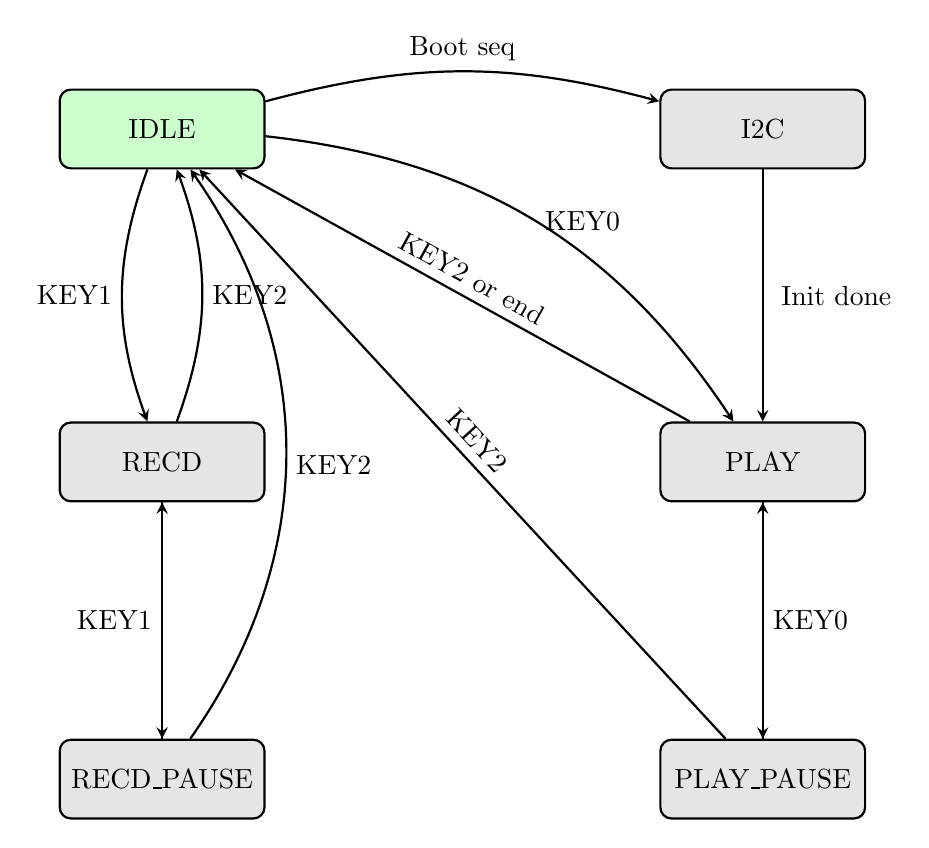
\begin{tikzpicture}[
  node distance=3.5cm and 3.2cm,
  >=stealth,
  thick,
  state/.style={rectangle, rounded corners, draw=black, fill=gray!20,
                minimum width=2.6cm, minimum height=1cm, text centered},
  initial/.style={fill=green!20}
]

% --- States ---
\node[state, initial]                     (IDLE)      {IDLE};
\node[state, right=5cm of IDLE]           (I2C)       {I2C};
\node[state, below=3.2cm of I2C]          (PLAY)      {PLAY};
\node[state, below=3cm of PLAY]         (PLAYPAUSE) {PLAY\_PAUSE};
\node[state, left=5cm of PLAY]            (RECD)      {RECD};
\node[state, below=3cm of RECD]         (RECDPAUSE) {RECD\_PAUSE};

% --- Transitions ---
\path[->]
  (IDLE) edge[bend left=15] node[above] {Boot seq} (I2C)
  (I2C) edge node[right, xshift=3pt] {Init done} (PLAY)
  (PLAY) edge node[above, sloped] {KEY2 or end} (IDLE)
  (PLAYPAUSE) edge node[above, sloped] {KEY2} (IDLE)

  (IDLE) edge[bend right=20] node[left] {KEY1} (RECD)
  (RECD) edge[bend right=20] node[right] {KEY2} (IDLE)
  (RECDPAUSE) edge[bend right=35] node[right, yshift=-4pt] {KEY2} (IDLE)

  (RECD) edge node[right] {} (RECDPAUSE)
  (RECDPAUSE) edge node[left] {KEY1} (RECD)

  (IDLE) edge[bend left=25] node[right] {KEY0} (PLAY)
  (PLAY) edge node[right] {} (PLAYPAUSE)
  (PLAYPAUSE) edge node[right] {KEY0} (PLAY);

\end{tikzpicture}


\caption{Main System State Machine}
\label{fig:main_fsm}
\end{figure}

\subsubsection{Initialization Sequence}

Upon power-on or reset, the system automatically performs initialization:

\begin{enumerate}
    \item System starts in \texttt{S\_IDLE}
    \item If \texttt{boot\_done\_r} is false, automatically transitions to \texttt{S\_I2C}
    \item I2C initialization configures WM8731 codec registers
    \item Upon completion, transitions to \texttt{S\_CLEAN}
    \item SRAM is cleared by writing zeros to all addresses
    \item Returns to \texttt{S\_IDLE} and sets \texttt{boot\_done\_r} flag
    \item System is ready for user operations
\end{enumerate}

\subsection{Submodule FSMs}

\subsubsection{AudDSP FSM}

The AudDSP module implements a three-state FSM for playback control:

\begin{verbatim}
States:
- S_IDLE:   Idle, waiting for start signal
- S_PLAY:   Active playback with speed/effect processing
- S_PAUSE:  Playback paused, maintaining current state
\end{verbatim}

\noindent
\textbf{Key Operations in the S\_PLAY State}:
\begin{itemize}
    \item Address generation based on speed mode (fast/slow/normal)
    \item Sample interpolation for slow playback
    \item Robot voice effect processing (when enabled)
    \item Synchronized to I2S clock domain via \texttt{daclrck\_pos\_edge}
\end{itemize}

\subsubsection{AudRecorder FSM}

The AudRecorder module implements a three-state FSM for recording:

\begin{verbatim}
States:
- IDLE:      Waiting for start signal
- RECORDING: Active recording, collecting I2S data
- PAUSED:    Recording paused
\end{verbatim}

\noindent
\textbf{Key Operations in the RECORDING State}:
\begin{itemize}
    \item Samples serial audio data on negative edge of \texttt{i\_bclk}
    \item Detects rising edge of \texttt{i\_lrc} to start new sample
    \item Collects 16 bits into shift register
    \item Writes to SRAM and increments address on sample completion
    \item Handles overflow condition when address reaches maximum
\end{itemize}

\subsubsection{I2cInitializer FSM}

The I2cInitializer implements a complex FSM for I2C protocol:

\begin{itemize}
    \item Handles START condition
    \item Bit-by-bit transmission of 3 bytes per register
    \item ACK/NACK detection after each byte
    \item STOP condition
    \item Repeats for 6 configuration registers
\end{itemize}

\subsection{Clock Domain Management}

The system operates across multiple clock domains, requiring careful synchronization:

\subsubsection{Clock Domains}

\begin{itemize}
    \item \textbf{12 MHz (i\_clk)}: 
        \begin{itemize}
            \item Main system clock
            \item Top FSM state machine
            \item LCD controller
            \item SRAM clearing module
        \end{itemize}
    
    \item \textbf{100 kHz (i\_clk\_100k)}: 
        \begin{itemize}
            \item I2C communication clock
            \item I2cInitializer module
        \end{itemize}
    
    \item \textbf{I2S Bit Clock (i\_AUD\_BCLK)}: 
        \begin{itemize}
            \item Audio data clock (typically 12.288 MHz)
            \item AudRecorder (negative edge sampling)
            \item AudDSP (main processing clock)
            \item AudPlayer (positive edge output)
        \end{itemize}
    
    \item \textbf{32 kHz (I2S LRCK)}: 
        \begin{itemize}
            \item Sample rate clock
            \item Synchronizes sample boundaries
            \item Triggers address updates
        \end{itemize}
\end{itemize}

\subsubsection{Synchronization Strategy}

\begin{itemize}
    \item Each module operates within its designated clock domain
    \item Cross-domain signals use edge detection for synchronization
    \item Control signals from 12 MHz domain are synchronized at module boundaries
    \item I2S modules sample/output on appropriate clock edges per WM8731 specification
    \item Address and data signals are registered to prevent metastability
\end{itemize}

\subsection{Hardware Scheduling Mechanism}

\subsubsection{Resource Sharing}

The system shares SRAM between multiple operations using multiplexers:

\begin{lstlisting}[language=Verilog]
// Address multiplexer based on current state
assign o_SRAM_ADDR = (state_r == S_RECD || state_r == S_RECD_PAUSE) ? addr_record : (state_r == S_CLEAN) ? addr_clean : addr_play;

// Data multiplexer
assign io_SRAM_DQ  = (state_r == S_RECD) ? data_record :
                     (state_r == S_CLEAN) ? data_clean : 16'hzzzz;
assign data_play   = io_SRAM_DQ;

// Write enable control
assign o_SRAM_WE_N = (state_r == S_RECD || state_r == S_CLEAN) ? 1'b0 : 1'b1;
\end{lstlisting}

\subsubsection{Operation Coordination}

The main FSM coordinates module operations:

\begin{itemize}
    \item \textbf{Recording Mode}: 
        \begin{itemize}
            \item Enables \texttt{rec\_start} signal to AudRecorder
            \item Routes \texttt{addr\_record} to SRAM address bus
            \item Routes \texttt{data\_record} to SRAM data bus
            \item Sets SRAM write enable
        \end{itemize}
    
    \item \textbf{Playback Mode}: 
        \begin{itemize}
            \item Enables \texttt{dsp\_start} signal to AudDSP
            \item AudDSP generates \texttt{addr\_play} based on speed mode
            \item SRAM data is read and fed to AudDSP
            \item Processed data flows to AudPlayer for output
        \end{itemize}
    
    \item \textbf{Clearing Mode}: 
        \begin{itemize}
            \item Activates Clean\_sram module
            \item Sequentially writes zeros to all SRAM addresses
            \item Completes initialization sequence
        \end{itemize}
\end{itemize}

\subsection{Real-time Performance}

The system maintains real-time audio processing through:

\begin{itemize}
    \item \textbf{Synchronized Operations}: Audio modules synchronized to I2S clock
    \item \textbf{Deterministic Timing}: FSM ensures predictable state transitions
    \item \textbf{Buffering}: SRAM provides buffer between recording and playback
    \item \textbf{Pipeline Processing}: DSP operations complete within sample period
    \item \textbf{Priority Management}: Recording and playback are mutually exclusive
\end{itemize}

\subsection{Summary}

The hardware scheduling mechanism successfully coordinates multiple concurrent operations through a hierarchical FSM structure. The design ensures:

\begin{itemize}
    \item Proper initialization sequence on startup
    \item Exclusive access to shared resources (SRAM)
    \item Real-time audio processing within timing constraints
    \item Flexible operation modes (record, play, pause)
    \item Robust state management with clear transitions
\end{itemize}



\section{Fitter Summary}
\section{Timing Analyzer}

\bibliographystyle{alpha}
\bibliography{sample}

\end{document}
